\loesung{
\begin{enumerate}[a)]
  \item Calculation of Pearson correlation coefficient of $x_1$ and $x_2$
  $$
 \rho(x_1, x_2) = \frac{\sum_{i = 1}^n (x_1^{(i)} - \overline{x}_1)(x_2^{(i)} - \overline{x}_2)}{\sqrt{\sum_{i = 1}^n (x_1^{(i)} - \overline{x}_1)^2} \sqrt{\sum_{i = 1}^n (x_2^{(i)} - \overline{x}_2)^2}}
  $$ 
   
  given the dataset

 \begin{table}[ht]
\centering
\begin{tabular}{rrrrrrrrrrrr|r}
\hline
& 1 & 2 & 3 & 4 & 5 & 6 & 7 & 8 & 9 & 10 & 11 & $\sum_{i = 1}^n$ \\ 
\hline
y & -7.90 & -6.08 & -3.74 & -1.18 & -1.23 & -0.55 & 0.05 & 0.88 & 4.74 & 2.93 & 2.55 & -9.53\\ 
x1 & -1.00 & -0.80 & -0.60 & -0.40 & -0.20 & 0.00 & 0.20 & 0.40 & 0.60 & 0.80 & 1.00 & 0 \\ 
x2 & 0.95 & 0.65 & 0.40 & 0.07 & 0.06 & 0.02 & 0.02 & 0.14 & 0.34 & 0.60 & 0.98 & 4.23 \\ 
\hline
\end{tabular}
\end{table}
 
 The individual differences to the means are
\begin{table}[h]
\centering
\begin{tabular}{rrrrrrrrrrrr}
  \hline
 & 1 & 2 & 3 & 4 & 5 & 6 & 7 & 8 & 9 & 10 & 11 \\ 
\hline
  $x_1^{(i)} - \overline{x}_1$ & -1.00 & -0.80 & -0.60 & -0.40 & -0.20 & 0.00 & 0.20 & 0.40 & 0.60 & 0.80 & 1.00 \\ 
  $x_2^{(i)} - \overline{x}_2$ & 0.57 & 0.27 & 0.02 & -0.31 & -0.32 & -0.36 & -0.36 & -0.24 & -0.04 & 0.22 & 0.6 \\ 
   \hline
\end{tabular}
\end{table}
  
     $$ 
    \begin{aligned}
  \rho(x_1, x_2) & = \frac{\sum_{i = 1}^n (x_1^{(i)} - \overline{x}_1)(x_2^{(i)} - \overline{x}_2)}{\sqrt{\sum_{i = 1}^n (x_1^{(i)} - \overline{x}_1)^2} \sqrt{\sum_{i = 1}^n (x_2^{(i)} - \overline{x}_2)^2}} \\
  & = \frac{-0.57 + -0.22 + -0.01 + 0.12 + -0.06 + 0 + -0.07 + -0.1 + -0.02 + 0.18 + 0.6}{2.41} = \frac{-0.03}{2.41} = -0.01
    \end{aligned}
  $$ 
  
  The Pearson correlation coefficient is close to 0 $\Rightarrow$ there is no \textbf{linear} relationship between $x_1$ and $x_2$.
  
  \item  The scatter plot reveals that there is a strong non-linear/quadratic relationship between $x_1$ and $x_2$. The Pearson correlation coefficients is not suitable
  for detecting non-linear relationships.
  
\begin{center}
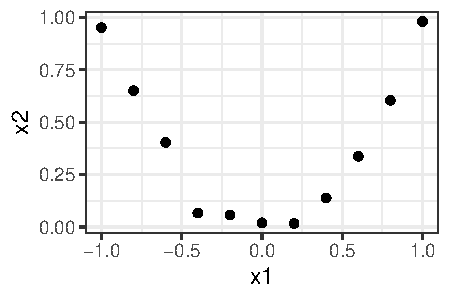
\includegraphics[width=\maxwidth]{figure/add_Points_x1_x2_sol.pdf}
\end{center}
 
  \item The p-value of $2.79 \times 10^{-5}$ (but also the adjusted $R^2$ value) reveals that there is a strong relationship between $x_1$ and $x_2$.
  The p-value does not reveal the shape of this relationship.
  
\end{enumerate}
}
